\documentclass[12pt, a4paper, oneside]{ctexart}
\usepackage{amsmath, amsthm, amssymb, bm, color, graphicx, geometry, hyperref, mathrsfs,extarrows, braket, booktabs, array}

\linespread{1.5}
%\geometry{left=2.54cm,right=2.54cm,top=3.18cm,bottom=3.18cm}
\geometry{left=1.84cm,right=1.84cm,top=2.18cm,bottom=2.18cm}
\newenvironment{problem}{\par\noindent\textbf{题目. }}{\bigskip\par}
\newenvironment{solution}{\par\noindent\textbf{解答. }}{\bigskip\par}
\newenvironment{note}{\par\noindent\textbf{注记. }}{\bigskip\par}

% 基本信息
\newcommand{\RQ}{\today} % 日期
\newcommand{\km}{最优化方法} % 科目
\newcommand{\bj}{强基数学002} % 班级
\newcommand{\xm}{吴天阳} % 姓名
\newcommand{\xh}{2204210460} % 学号

\begin{document}

%\pagestyle{empty}
\pagestyle{plain}
\vspace*{-15ex}
\centerline{\begin{tabular}{*5{c}}
    \parbox[t]{0.25\linewidth}{\begin{center}\textbf{日期}\\ \large \textcolor{blue}{\RQ}\end{center}} 
    & \parbox[t]{0.2\linewidth}{\begin{center}\textbf{科目}\\ \large \textcolor{blue}{\km}\end{center}}
    & \parbox[t]{0.2\linewidth}{\begin{center}\textbf{班级}\\ \large \textcolor{blue}{\bj}\end{center}}
    & \parbox[t]{0.1\linewidth}{\begin{center}\textbf{姓名}\\ \large \textcolor{blue}{\xm}\end{center}}
    & \parbox[t]{0.15\linewidth}{\begin{center}\textbf{学号}\\ \large \textcolor{blue}{\xh}\end{center}} \\ \hline
\end{tabular}}
\vspace*{4ex}

% 正文部分
\def\disp{\displaystyle}
\paragraph{第三章}
\paragraph{4.}设$\varphi(t)=e^{-t}+e^t$,区间为$[-1,1]$。

(1) 用$0.618$法极小化$\varphi(t)$。(计算两步)

(2) 用Fibonacci法极小化$\varphi(t)$。(计算两步)
\begin{solution}
    (1) 初始化:
    \begin{equation*}
        a_1 = -1,\ b_1 = 1,\ \lambda_1 = a_1+\frac{3-\sqrt{5}}{2}(b_1-a_1) = 2-\sqrt{5},\ \mu_1 = a_1+\frac{\sqrt{5}-1}{2}(b_1-a_1) = \sqrt{5} - 2
    \end{equation*}

    第一步:由于$\varphi(t)$为偶函数,所以$\varphi(\lambda_1) = \varphi(\mu_1)$,于是
    \begin{equation*}
        a_2=a_1=-1,\ b_2=\mu_1=\sqrt{5}-2,\ \mu_2=\lambda_1 = 2-\sqrt{5}, \lambda_2 = a_2+\frac{3-\sqrt{5}}{2}(b_2-a_2) = 2\sqrt{5}-5
    \end{equation*}

    第二步:由于$2.285\approx\varphi(\lambda_2) > \varphi(\mu_2)\approx 2.056$,所以极小化值为$\varphi(\mu_2)\approx 2.056$。

    (2) 初始化:取$n = 4$,则$\disp a_1 = -1,\ b_1 = 1,\ \lambda_1 = a_1 + \frac{1}{3}(b_1-a_1) = -\frac{1}{3},\ \mu_1 = a_1+\frac{2}{3}(b_1-a_1) = \frac{1}{3}$

    第一步:由于$\varphi(\lambda_1) = \varphi(\mu_1)$,于是
    \begin{equation*}
        a_2 = a_1 = -1,\ b_2=\mu_1=\frac{1}{3},\ \mu_2 = \lambda_1 = -\frac{1}{3},\ \lambda_2 = a_2+\frac{1}{2}(b_2-a_2) = -\frac{1}{3}
    \end{equation*}

    第二步:由于$\mu_2 = \lambda_2$,于是极小化值为$\varphi(\mu_2) \approx 2.112$。
\end{solution}
\paragraph{6.}设$\varphi(t) = 1-te^{-t^2}$,区间为$[0,1]$。试用三点二次插值法极小化$\varphi(t)$。(计算一步)
\begin{solution}
    设$x_1=0,\ x_2 = 0.5,\ x_3 = 1$,下面列出三阶差商表
    \renewcommand\arraystretch{0.8} % 设置表格高度为原来的0.8倍
    \begin{table}[!htbp] % table标准
        \centering % 表格居中
        \begin{tabular}{p{1cm}<{\centering}p{3cm}<{\centering}p{4cm}<{\centering}p{5cm}<{\centering}} % 设置表格宽度
        %\begin{tabular}{cccc}
            \toprule
            $x_i$ & $\varphi[x_i]$ & $\varphi[x_i,x_{i+1}]$ & $\varphi[x_i,x_{i+1},x_{i+2}]$ \\
            \midrule
            $x_1$ & $1$ &                  &                          \\
            $x_2$ & $1-\frac{1}{2}e^{-\frac{1}{4}}$ & $-e^{-\frac{1}{4}}$        &                          \\
            $x_3$ & $1-e^{-1}$ & $e^{-\frac{1}{4}}-2e^{-1}$ & $2e^{-\frac{1}{4}}-2e^{-1}$\\
            \bottomrule
        \end{tabular}
    \end{table}

    由Newton插值多项式可知
    \begin{equation*}
        \begin{aligned}
            N_2(x) = 1-e^{-\frac{1}{4}}x+(2e^{-\frac{1}{4}}-2e^{-1})x(x-\frac{1}{2}) = (2e^{-\frac{1}{4}}-2e^{-1})x^{2}+(-2e^{-\frac{1}{4}}+e^{-1})x+1
        \end{aligned}
    \end{equation*}
    则$\disp \overline{x}=\frac{2e^{-\frac{1}{4}}-e^{-1}}{4(e^{-\frac{1}{4}}-e^{-1})}\approx 0.7238 > x_2$,又由于$0.61\approx \varphi(x_2) >\overline{\varphi} = \varphi(\overline{x})\approx 0.57$,所以令$x_1\Leftarrow \overline{x},\ \varphi(x_1) \Leftarrow \overline{\varphi}$,极小化值为$\overline{\varphi}\approx 0.57$。

\end{solution}
\paragraph{第四章}
\paragraph*{1.}设$\disp f(x) = \frac{3}{2}x_1^2+\frac{1}{2}x_2^2-x_1x_2-2x_1$,设初始点$x^{(0)} = (-2, 4)^T$。试用最速下降法和牛顿法极小化$f(x)$。(计算两步)
\begin{solution}
    最速下降法:已知$\nabla f = [3x_1-x_2-2,x_2-x_1]^T$,$x^{(0)} = (-2, 4)^T$。
    
    第一步:$d_0 = -g_0 = -\nabla f(x^{(0)}) = [12, -6]^T$,求线性步长因子
    \begin{equation*}
        \nabla f(x^{(0)} + \alpha_0d_0)^Td_0 = \nabla f(-2+12\alpha_0, 4-6\alpha_0)^T\left[\begin{matrix}
            12\\-6
        \end{matrix}\right] = -5+16\alpha_0 = 0
    \end{equation*}
    则$\disp \alpha_0 = \frac{5}{17}$,于是$\disp x^{(1)} = x^{(0)} + \alpha_0d_0 = (\frac{26}{17},\frac{38}{17})^T$。

    第二步:$ d_1 = -g_1 = -\nabla f(x^{(1)}) = -\left[\frac{6}{17}, \frac{12}{17}\right]^T$,求线性步长因子
    \begin{equation*}
        \nabla f(x^{(1)}+\alpha_1d_1)^Td_1 = \nabla f\left(\frac{26}{17}-\frac{6}{17}\alpha_1,\frac{38}{17}-\frac{12}{17}\alpha_1\right)^T\left[\begin{matrix}
            -\frac{6}{17}\\-\frac{12}{17}
        \end{matrix}\right] = \left(\frac{6}{17}\right)^2(3\alpha_1-5) = 0
    \end{equation*}
    则$\disp \alpha_1 = \frac{5}{3}$,于是$\disp x^{(2)} = x^{(1)} + \alpha_1d_1 = \left(\frac{16}{17},\frac{18}{17}\right)^T$,所以通过最速下降法两步得到的极小化值为
    \begin{equation*}
        f(x^{(2)}) = \frac{3}{2}\cdot \left(\frac{16}{17}\right)^2+\frac{1}{2}\left(\frac{18}{17}\right)^2-\frac{16}{17}\cdot \frac{18}{17}-2\cdot \frac{16}{17} = -\frac{286}{289} \approx -0.9896
    \end{equation*}

    牛顿法:已知$\disp\nabla^2f(x) = \left[\begin{matrix}
        3&-1\\-1&1
    \end{matrix}\right]$,$x^{(0)} = (-2,4)^T$,则
    \begin{equation*}
        G_0d_0 = -g_0\Rightarrow \left[\begin{matrix}
            -3&-1\\-1&1
        \end{matrix}\right]d_0=\left[\begin{matrix}
            12\\-6
        \end{matrix}\right]\Rightarrow d_0 = \left[\begin{matrix}
            3\\-3
        \end{matrix}\right]
    \end{equation*}
    求线性步长因子
    \begin{equation*}
        \nabla f(x^{(0)} + \alpha_0d_0)^Td_0 = \nabla f(-2+3\alpha_0, 4-3\alpha_0)^T\left[\begin{matrix}
            3\\-3
        \end{matrix}\right] = 54(\alpha_0-1) = 0
    \end{equation*}
    则$\alpha_0 = 1$,于是$x^{(1)} = x^{(0)} + \alpha_0d_0 = (1, 1)^T$,由于$g_1 = \nabla f(x^{(1)}) = \mathbf{0}$,所以$f(x)$的极小化值为$f(x^{(1)}) = -1$。
\end{solution}
\paragraph*{定理 4.3.3.}设$x_0\in\mathbb{R}^n$是任意初始点。对于极小化二次函数$\disp \frac{1}{2}x^TGx-b^Tx$,共轭方向至多经$n$步精确线性搜索终止;且每一$x_{i+1}$都是$f(x)$在$x_0$和方向$d_0,\cdots, d_i$所张成的线性流形$\disp\{x:x=x_0+\sum_{j=0}^i\alpha_jd_j,\ \forall \alpha_j\}$中的极小点。
\begin{proof}
    设$U = \disp\{x:x=x_0+\sum_{j=0}^i\alpha_jd_j,\ \forall \alpha_j\}$,则$\disp x_{i+1} = \min_{x\in U}f(x)$等价于
    \begin{equation*}
        \nabla f(x_{i+1}) = 0\iff [g_{i+1}^Td_1, g_{i+1}^Td_2,\cdots, g_{i+1}^Td_i] = 0
    \end{equation*}
    所以,只需证明$\forall 1\leqslant i \leqslant n$,有$g_i^Td_j = 0\ (\forall 0\leqslant j < i)$成立,由于
    \begin{equation*}
        g_{k+1}-g_k = G(x_{k+1}-x_k) = \alpha Gd_k\ \text{且}\ g_{k+1}^Td_k = 0
    \end{equation*}
    则,任意的$j < i$有
    \begin{equation*}
        \begin{aligned}
            g_i^Td_j =&\ (g_{j+1} + (g_i-g_{i-1}+g_{i-1}-g_{i-2}+\cdots+g_{j+2}-g_{j+1}))^Td_j\\
            =&\ \left(g_{j+1}+\sum_{k=j+1}^{i-1}\alpha_kd_j^TGd_k\right)^T d_j = g_{j+1}d_j+\sum_{k=j+1}^{i-1}\alpha_kd_j^TGd_k\\
            =&\ 0\quad\text{(第一式由于精确线性搜索为0,第二式由于共轭性为0)}
        \end{aligned}
    \end{equation*}
    由于$\mathbb{R}^n$空间可以视为由$n$个共轭向量所张成的,当$i = n$时,有$g_n^Td_j = 0\ (j=0,1,\cdots, n-1)$,所以$g_n \equiv 0$,所以共轭方向法至多经$n$步精确线性搜索终止。
\end{proof}
\paragraph*{4.}证明:当极小化正定二次函数时,共轭梯度法FR公式,PRP公式和Dixon公式是等价的。
\begin{proof}
    设正定二次函数为$\disp f(x)=\frac{1}{2}x^TGx-b^Tx$,第$k$步的搜索方向为$d_k=-g_k+\beta_{k-1}d_{k-1}$,由精确线性搜索可知$g_{k+1}^Td_k = 0$,则$g_{k+1}^T(-g_k+\beta_{k-1}d_{k-1}) = 0$,通过\textbf{定理4.3.3}可知$g_{k+1}^Tg_k = \beta_{k-1}g_{k+1}^Td_{k-1} = 0$,于是
    \begin{equation*}
        \begin{aligned}
            (\text{Dixon公式})\quad \beta_{k-1} = -\frac{g_k^Tg_k}{d_{k-1}^Tg_{k-1}} =&\ -\frac{g_k^Tg_k}{(-g_{k-1}+\beta_{k-2}d_{k-2})^Tg_{k-1}} \xlongequal{\text{精确线性搜索条件}}\frac{g_k^Tg_k}{g_{k-1}^Tg_{k-1}}\quad(\text{FR公式})\\
            =&\ \frac{g_k^Tg_k+g_k^Tg_{k-1}}{g_{k-1}^Tg_{k-1}} = \frac{g_k^T(g_k-g_{k-1})}{g_{k-1}^Tg_{k-1}}\quad(\text{PRP公式})
        \end{aligned}
    \end{equation*}
\end{proof}

% 下面给一些功能的写法
\iffalse
% 图片模板
\centerline{
    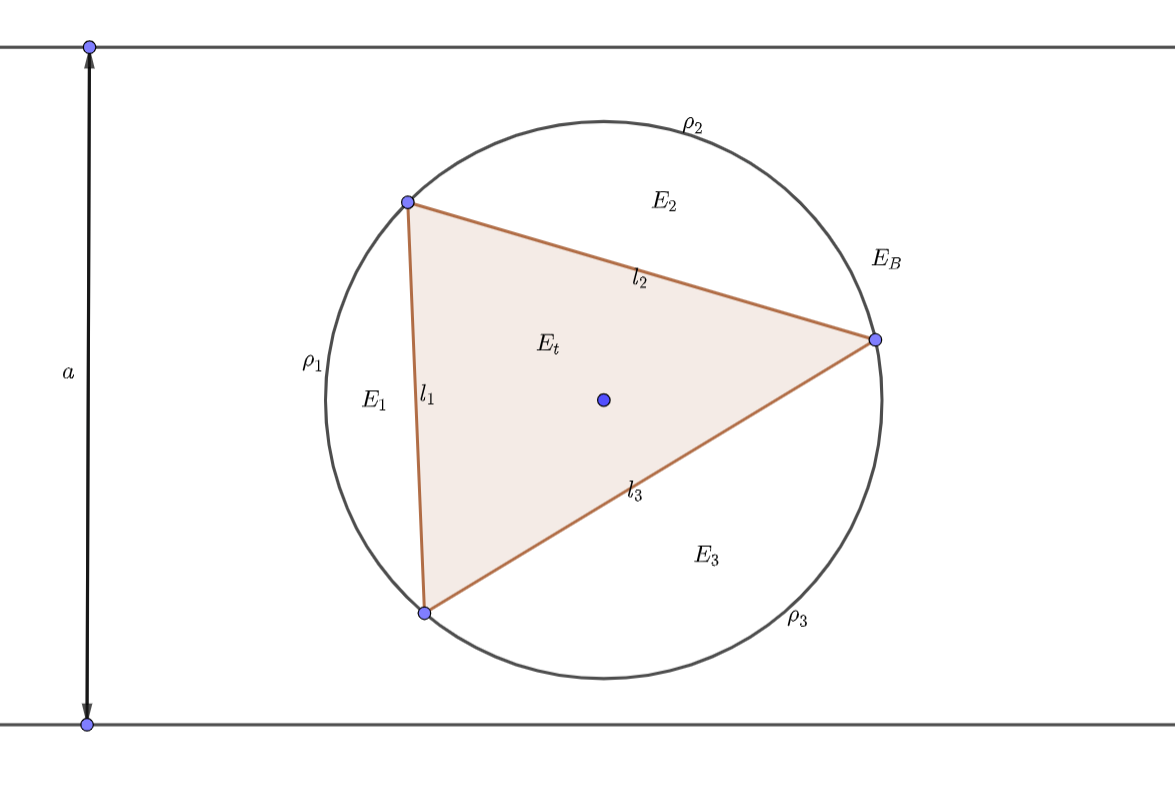
\includegraphics[width=0.8\textwidth]{figure.png}
}
% 表格模板
\renewcommand\arraystretch{0.8} % 设置表格高度为原来的0.8倍
\begin{table}[!htbp] % table标准
    \centering % 表格居中
    \begin{tabular}{p{1cm}<{\centering}p{1cm}<{\centering}p{3cm}<{\centering}p{5cm}<{\centering}} % 设置表格宽度
    %\begin{tabular}{cccc}
        \toprule
        $x_i$ & $f[x_1]$ & $f[x_i,x_{i+1}]$ & $f[x_i,x_{i+1},x_{i+2}]$ \\
        \midrule
        $x_0$ & $f(x_0)$ &                  &                          \\
        $x_0$ & $f(x_0)$ & $f'(x_0)$        &                          \\
        $x_0$ & $f(x_1)$ & $\frac{f(x_1)-f(x_0)}{x_1-x_0}$ & $\frac{f(x_1)-f(x_0)}{(x_1-x_0)^2}-\frac{f'(x_0)}{x_1-x_0}$\\
        \bottomrule
    \end{tabular}
\end{table}

\def\Log{\text{Log}} % 一个简单的宏定义
$\Log$ % 调用方法
\fi

\end{document}